\documentclass[12pt]{article}

\usepackage[margin=1in]{geometry}
\usepackage{amsmath,amsthm,amssymb}
\usepackage{enumitem}
\usepackage{physics}
\usepackage{subcaption}
\usepackage{graphicx}
\usepackage[style=numeric,sorting=none]{biblatex}
\addbibresource{refs.bib}
\graphicspath{ {./images/} }

\newcommand{\chrissym}[3]{\Gamma_{#2#3}^#1}

\begin{document}
\title{(2+1)-Dimensional Black Holes}
\author{Sean Ericson \\ Phys 610 Final}
\maketitle

\section{Introduction}
Black holes in our usual (3+1)-dimensional spacetime are well-studied and known to posses several interesting properties. They are primarily defined by the presence of an ``event horizon'': a hypersurface that divides spacetime into points that are connected to spacial infinity by timelike paths and those that are not. Observers approaching the horizon (from the infinity-connected side) on timelike paths will cross will cross it in a finite time. However, a second observer watching the first ``from infinity'' (i.e. sufficiently far away so as to experience negligible spacetime curvature) will see it take an infinite amount of time for them to fall in, becoming more and more redshifted as they asymptotically approach the horizon. While the horizon is the defining feature of the black hole, they typically contain within the horizon a point (or a ring in the case of a spinning black hole) where spacetime curvature diverges, known as the singularity. Additionally, it turns out that the only parameters needed to completely specify a black hole are its mass, charge, and angular momentum (this is known as the ``No Hair'' theorem) \cite{carroll}. The solution to the Einstein equation for a non-rotating, uncharged black hole is given by the Schwarzschild metric:
\begin{equation}
    \dd s^2 = -\left(1-\frac{2GM}{r}\right)\dd t^2 + \left(1-\frac{2GM}{r}\right)^{-1} \dd r^2 + r^2 \dd\Omega^2,
\end{equation}
Where $G$ is the gravitational constant and $M$ is the mass of the black hole. For a charged, non-rotating black hole the solution is the Reissner-Nordstr{\"o}m metric:
\begin{equation}
    \dd s^2 = -\Delta \dd t^2 + \Delta^{-1}\dd r + r^2 \dd\Omega^2; \quad \Delta = 1 - \frac{2GM}{r} + \frac{GQ^2}{r^2},
\end{equation}
where $Q$ is the electric charge of the black hole. A rotating, non-charged black hole is given by the Kerr metric:
\begin{equation}
    \dd s^2 = -\left(1 - \frac{2GM}{\rho^2}\right)\dd t^2 - \frac{4GMar\sin^2\theta}{\rho^2}\dd t \dd \phi + \frac{\rho^2}{\Delta}\dd r^2 + \rho^2 \dd \theta^2 + \frac{\sin^2\theta}{\rho^2}\left[(r^2 + a^2)^2 - a^2\Delta\sin^2\theta\right]\dd\phi^2
\end{equation}
where 
\[ \Delta = r^2 - 2GMr + a^2; \quad \rho^2 = r^2 + a^2\cos^2\theta, \]
and $a = J/M$ is the angular momentum per unit mass. The most general solution (charged and rotating) is obtained simply by adding the term from the Reissner-Nordstr{\"o}m metric containing the charge to the definition of $\Delta$ in the Kerr metric.


\section{General Relativity in (2+1)-Dimensions}
\subsection{Degrees of freedom}
Einstein's equation in $d+1$ spacetime dimensions can be written \cite{cornish}
\begin{equation}
    R_{\mu\nu} - \frac{1}{2}Rg_{\mu\nu} + \Lambda g_{\mu\nu} = \frac{d-1}{d-2}G_dS_dT_{\mu\nu},
\end{equation}
where $G_d$ is the gravitational constant generalized to $d$-dimensions and $S_d$ is the area of the unit $d$-sphere. This form produces a theory with a correct Newtonian limit for $d\geq3$, but clearly something goes wrong for $d<3$. In fact, it turns out that there is no Newtonian limit for General Relativity in one or two spatial dimensions. We can see this more easily by considering the number of degrees of freedom. The Einstein equation relates the traceless part of the Riemann tensor to the stress-energy tensor. Specifically, it states that outside of a distribution of matter/energy (i.e. vacuum) the traceless part of the Riemann tensor vanishes. Therefore the only remaining degrees of freedom must lie in the non-traceless part of the Riemann tensor, which is encapsulated by the Weyl tensor. The Weyl tensor has \[ \frac{1}{12}(d+1)(d+2)(d+3)(d-2) \] independent components. Hence, spacetime curvature in 2+1 dimensions outside of sources is trivial: either flat, de Sitter or anti-de Sitter, depending on the sign of $\Lambda$. However, it turns out that matter-energy sources can have nontrivial \textit{topological} effects on the spacetime.

\subsection{The Topology of (2+1)-d Spacetime}
Consider the case of a point mass in $(2+1)-d$ spacetime with zero cosmological constant. The point mass introduces a \textit{conical} singularity in the spatial part of the spacetime. The metric for such a case is given by \cite{cornish}
\begin{equation}
    \dd s^2 = -\dd t^2 + \frac{1}{1-2GM}\dd r^2 + r^2 \dd\phi^2.
\end{equation}
Such a geometry is characterized by a ``deficit angle'' $\alpha = 2\pi\left(1 - \sqrt{1 - 2GM}\right)$, which corresponds to the angle of the conical global geometry depicted in Figure 1.
\begin{figure}[h]
    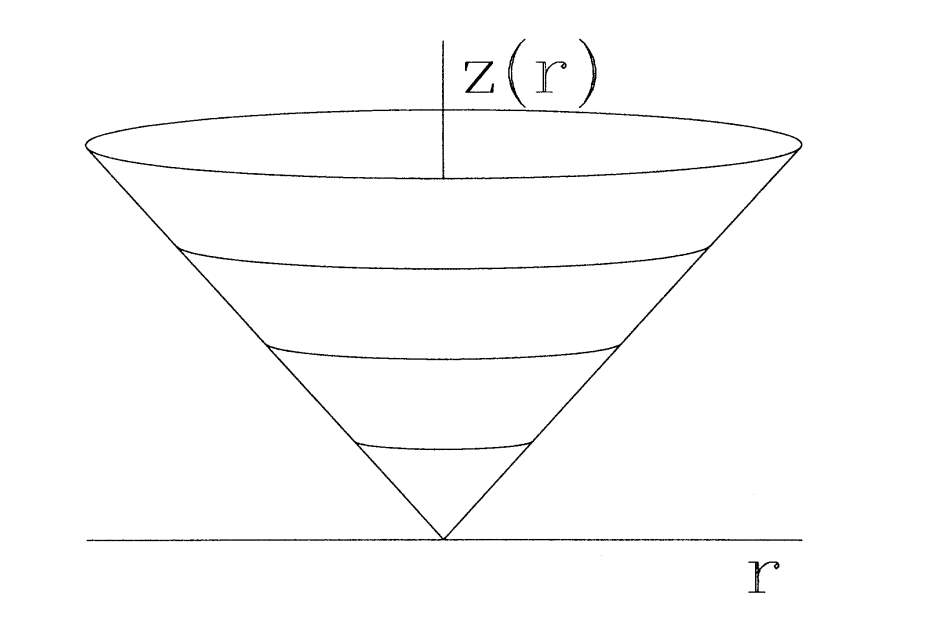
\includegraphics[scale=0.7]{cone1.PNG}
    \centering
    \caption{Embedding of the spatial part of the spacetime geometry of a point mass in 3D space. (From \cite{2})}
    \label{fig1}
\end{figure}

\section{Black Holes in (2+1)-Dimensions}
The surprising fact that Einstein's equation in $(2+1)-d$ permits a black hole solution was first identified by Ba{\~n}ados, Teitelboim and Zanelli in 1992 \cite{banados92}, and they are therefore known as BTZ black holes. Their solution assumes a negative cosmological constant, but subsequent work has shown that similar results can be achieved in spacetime with $\Lambda=0$ given a particular nontrivial type of matter field \cite{chan}.

\subsection{Derivation}
BTZ begin their derivation by recasting the Hilbert action into Hamiltonian form
\begin{align}
    I_\text{H} &= \int \dd^3x\sqrt{-g}\left(R - 2\Lambda\right) - \frac{1}{4}F_{\mu\nu}F^{\mu\nu} \\
    \to I &= \int\dd t\dd^3x\left(\pi^{ij}\dot{g}_{ij} + \mathcal{E}^i\dot{A}_i - N^\perp\mathcal{H}_\perp - N^i\mathcal{H}_i + A_0\partial_i\mathcal{E}^i\right) \nonumber
\end{align}
where
\begin{align}
    \mathcal{H}_\perp &= g^{-1/2}(\pi^{ij}\pi_{ij} -(\pi_i^i)^2) - g^{1/2}(R-2\Lambda), \\
    \mathcal{H}_i &= -2\Delta_j\pi_i^j + \mathcal{E}^jF_{ij}, \nonumber
\end{align}
the $N^\perp$, $N^i$ are lagrange multipliers, and the canonical variables are the metric and the vector potential, along with their conjugates ($\pi^{ij}$ and $\mathcal{E}^i$, respectively). Also, units have been adopted in which $G = 1/16\pi$. The cosmological constant has units of inverse length squared, and it will be convenient to switch to working with it's associated squared-length: $\Lambda \to -l^{-2}$. Note that in 2 spatial dimensions (and without magnetic monopoles) the magnetic field $\mathcal{B}$ is a scalar rather than a vector, and is related to the field strength tensor by \[ F_{ij} = \epsilon_{ij}\mathcal{B}. \]

Demanding a rotationally symmetric, time translation-invariant metric implies the form
\begin{equation}
    \dd s^2 = -N^2(r)f^2(r)\dd t^2 + f^{-2}(r)\dd r^2 + r^2\left(\dd \phi^2 + N^\phi(r)\dd t\right)^2
\end{equation}
Extremizing the action (6) results in differential equations for the functions $N(r)$, $f(r)$ and $N^\phi(r)$. The constants of integration from these equations are themselves functions of the mass, charge, and angular momentum of the black hole.

\subsection{Properties}
Charged, non-rotating (2+1)-d black holes exhibit an inner and outer horizon similar to their (3+1)-d counterparts.

\vspace{10em}
I'm sorry; it turns out an extra day wasn't enough to really cover this as much as I had liked too. I found all these nice sources, but it turns out that there's a lot more to 2+1d GR than I had initially thought. \\
\noindent Lectures in (2+1)D Gravity (Carlip '95) \cite{carlipLec} \\
Gravitation in (2+1)D (Cornish, N. J. and Frankel, N. E. '91) \cite{cornish} \\
Gravitationally collapsing dust in 2 + 1 dimensions (Mann, R. B. and Ross, S. F. '93) \cite{mann93}
Charged rotating black hole in three spacetime dimensions (Martínez, Cristián and Teitelboim, Claudio and Zanelli, Jorge '00)\cite{martinez} \\
Black hole in three-dimensional spacetime (Bañados, Máximo and Teitelboim, Claudio and Zanelli, Jorge '92) \cite{banados92} \\
Geometry of the 2+1 black hole (Bañados, Máximo and Henneaux, Marc and Teitelboim, Claudio and Zanelli, Jorge '93) \cite{banados93} \\
The (2 + 1)-dimensional black hole (Carlip, S '95) \cite{carlip95} \\
Static Charged Black Holes in (2+1) Dimensional Dilaton Gravity (K.C.K Chan '94) \cite{chan} \\

\printbibliography
\end{document}